\documentclass{article}
\usepackage[utf8]{inputenc}
\usepackage[top=1in]{geometry}
\usepackage{graphicx}
\usepackage{booktabs}
\usepackage{amsmath}
\usepackage{amsthm}
\usepackage[only]{excludeonly}
\usepackage{fancyhdr}
\usepackage{tikz}
\usetikzlibrary{circuits.logic.US,positioning,calc} 
\usepackage[american]{circuitikz}

\usepackage{enumitem,amssymb}
\newlist{todolist}{itemize}{2}
\setlist[todolist]{label=$\square$}
\usepackage{pifont}
\newcommand{\cmark}{\ding{51}}%
\newcommand{\xmark}{\ding{55}}%
\newcommand{\done}{\rlap{$\square$}{\raisebox{2pt}{\large\hspace{1pt}\cmark}}%
  \hspace{-2.5pt}}
\newcommand{\wontfix}{\rlap{$\square$}{\large\hspace{1pt}\xmark}}

% https://tex.stackexchange.com/questions/140567/drawing-karnaughs-maps-in-latex
\usepackage{tikz}
\usetikzlibrary{matrix,calc}

%isolated term
%#1 - Optional. Space between node and grouping line. Default=0
%#2 - node
%#3 - filling color
\newcommand{\implicantsol}[3][0]{
    \draw[rounded corners=3pt, fill=#3, opacity=0.3] ($(#2.north west)+(135:#1)$) rectangle ($(#2.south east)+(-45:#1)$);
    }


%internal group
%#1 - Optional. Space between node and grouping line. Default=0
%#2 - top left node
%#3 - bottom right node
%#4 - filling color
\newcommand{\implicant}[4][0]{
    \draw[rounded corners=3pt, fill=#4, opacity=0.3] ($(#2.north west)+(135:#1)$) rectangle ($(#3.south east)+(-45:#1)$);
    }

%group lateral borders
%#1 - Optional. Space between node and grouping line. Default=0
%#2 - top left node
%#3 - bottom right node
%#4 - filling color
\newcommand{\implicantcostats}[4][0]{
    \draw[rounded corners=3pt, fill=#4, opacity=0.3] ($(rf.east |- #2.north)+(90:#1)$)-| ($(#2.east)+(0:#1)$) |- ($(rf.east |- #3.south)+(-90:#1)$);
    \draw[rounded corners=3pt, fill=#4, opacity=0.3] ($(cf.west |- #2.north)+(90:#1)$) -| ($(#3.west)+(180:#1)$) |- ($(cf.west |- #3.south)+(-90:#1)$);
}

%group top-bottom borders
%#1 - Optional. Space between node and grouping line. Default=0
%#2 - top left node
%#3 - bottom right node
%#4 - filling color
\newcommand{\implicantdaltbaix}[4][0]{
    \draw[rounded corners=3pt, fill=#4, opacity=0.3] ($(cf.south -| #2.west)+(180:#1)$) |- ($(#2.south)+(-90:#1)$) -| ($(cf.south -| #3.east)+(0:#1)$);
    \draw[rounded corners=3pt, fill=#4, opacity=0.3] ($(rf.north -| #2.west)+(180:#1)$) |- ($(#3.north)+(90:#1)$) -| ($(rf.north -| #3.east)+(0:#1)$);
}

%group corners
%#1 - Optional. Space between node and grouping line. Default=0
%#2 - filling color
\newcommand{\implicantcantons}[2][0]{
    \draw[rounded corners=3pt, opacity=.3] ($(rf.east |- 0.south)+(-90:#1)$) -| ($(0.east |- cf.south)+(0:#1)$);
    \draw[rounded corners=3pt, opacity=.3] ($(rf.east |- 8.north)+(90:#1)$) -| ($(8.east |- rf.north)+(0:#1)$);
    \draw[rounded corners=3pt, opacity=.3] ($(cf.west |- 2.south)+(-90:#1)$) -| ($(2.west |- cf.south)+(180:#1)$);
    \draw[rounded corners=3pt, opacity=.3] ($(cf.west |- 10.north)+(90:#1)$) -| ($(10.west |- rf.north)+(180:#1)$);
    \fill[rounded corners=3pt, fill=#2, opacity=.3] ($(rf.east |- 0.south)+(-90:#1)$) -|  ($(0.east |- cf.south)+(0:#1)$) [sharp corners] ($(rf.east |- 0.south)+(-90:#1)$) |-  ($(0.east |- cf.south)+(0:#1)$) ;
    \fill[rounded corners=3pt, fill=#2, opacity=.3] ($(rf.east |- 8.north)+(90:#1)$) -| ($(8.east |- rf.north)+(0:#1)$) [sharp corners] ($(rf.east |- 8.north)+(90:#1)$) |- ($(8.east |- rf.north)+(0:#1)$) ;
    \fill[rounded corners=3pt, fill=#2, opacity=.3] ($(cf.west |- 2.south)+(-90:#1)$) -| ($(2.west |- cf.south)+(180:#1)$) [sharp corners]($(cf.west |- 2.south)+(-90:#1)$) |- ($(2.west |- cf.south)+(180:#1)$) ;
    \fill[rounded corners=3pt, fill=#2, opacity=.3] ($(cf.west |- 10.north)+(90:#1)$) -| ($(10.west |- rf.north)+(180:#1)$) [sharp corners] ($(cf.west |- 10.north)+(90:#1)$) |- ($(10.west |- rf.north)+(180:#1)$) ;
}

%Empty Karnaugh map 4x4
\newenvironment{Karnaugh}[2]%
{
\begin{tikzpicture}[baseline=(current bounding box.north),scale=0.8]
\draw (0,0) grid (4,4);
\draw (0,4) -- node [pos=0.7,above right,anchor=south west] {#1} node [pos=0.7,below left,anchor=north east] {#2} ++(135:1);
%
\matrix (mapa) [matrix of nodes,
        column sep={0.8cm,between origins},
        row sep={0.8cm,between origins},
        every node/.style={minimum size=0.3mm},
        anchor=2.center,
        ampersand replacement=\&] at (0.5,0.5)
{
                       \& |(c00)| 00         \& |(c01)| 01         \& |(c11)| 11         \& |(c10)| 10         \& |(cf)| \phantom{00} \\
|(r00)| 00             \& |(0)|  \phantom{0} \& |(4)|  \phantom{0} \& |(12)|  \phantom{0} \& |(8)|  \phantom{0} \&                     \\
|(r01)| 01             \& |(1)|  \phantom{0} \& |(5)|  \phantom{0} \& |(13)|  \phantom{0} \& |(9)|  \phantom{0} \&                     \\
|(r11)| 11             \& |(3)| \phantom{0} \& |(7)| \phantom{0} \& |(15)| \phantom{0} \& |(11)| \phantom{0} \&                     \\
|(r10)| 10             \& |(2)|  \phantom{0} \& |(6)|  \phantom{0} \& |(14)| \phantom{0} \& |(10)| \phantom{0} \&                     \\
|(rf) | \phantom{00}   \&                    \&                    \&                    \&                    \&                     \\
};
}%
{
\end{tikzpicture}
}

%Empty Karnaugh map 2x4
\newenvironment{Karnaughvuit}%
{
\begin{tikzpicture}[baseline=(current bounding box.north),scale=0.8]
\draw (0,0) grid (4,2);
\draw (0,2) -- node [pos=0.7,above right,anchor=south west] {AB} node [pos=0.7,below left,anchor=north east] {C} ++(135:1);
%
\matrix (mapa) [matrix of nodes,
        column sep={0.8cm,between origins},
        row sep={0.8cm,between origins},
        every node/.style={minimum size=0.3mm},
        anchor=1.center,
        ampersand replacement=\&] at (0.5,0.5)
{
                      \& |(c00)| 00         \& |(c01)| 01         \& |(c11)| 11         \& |(c10)| 10         \& |(cf)| \phantom{00} \\
|(r00)| 0             \& |(0)|  \phantom{0} \& |(2)|  \phantom{0} \& |(6)|  \phantom{0} \& |(4)|  \phantom{0} \&                     \\
|(r01)| 1             \& |(1)|  \phantom{0} \& |(3)|  \phantom{0} \& |(7)|  \phantom{0} \& |(5)|  \phantom{0} \&                     \\
|(rf) | \phantom{00}  \&                    \&                    \&                    \&                    \&                     \\
};
}%
{
\end{tikzpicture}
}

%Empty Karnaugh map 2x2
\newenvironment{Karnaughquatre}%
{
\begin{tikzpicture}[baseline=(current bounding box.north),scale=0.8]
\draw (0,0) grid (2,2);
\draw (0,2) -- node [pos=0.7,above right,anchor=south west] {A} node [pos=0.7,below left,anchor=north east] {B} ++(135:1);
%
\matrix (mapa) [matrix of nodes,
        column sep={0.8cm,between origins},
        row sep={0.8cm,between origins},
        every node/.style={minimum size=0.3mm},
        anchor=1.center,
        ampersand replacement=\&] at (0.5,0.5)
{
          \& |(c00)| 0          \& |(c01)| 1  \\
|(r00)| 0 \& |(0)|  \phantom{0} \& |(2)|  \phantom{0} \\
|(r01)| 1 \& |(1)|  \phantom{0} \& |(3)|  \phantom{0} \\
};
}%
{
\end{tikzpicture}
}

%Defines 8 or 16 values (0,1,X)
\newcommand{\contingut}[1]{%
\foreach \x [count=\xi from 0]  in {#1}
     \path (\xi) node {\x};
}

%Places 1 in listed positions
\newcommand{\minterms}[1]{%
    \foreach \x in {#1}
        \path (\x) node {1};
}

%Places 0 in listed positions
\newcommand{\maxterms}[1]{%
    \foreach \x in {#1}
        \path (\x) node {0};
}

%Places X in listed positions
\newcommand{\indeterminats}[1]{%
    \foreach \x in {#1}
        \path (\x) node {X};
}

% Places m_{x} in listed positions
\newcommand{\phminterms}[1]{%
  \foreach \x in {#1}
  \path (\x) node {$m_{\x}$};
}

% Places m_{16+x} in listed positions
\newcommand{\phmintermssixt}[1]{%
  \foreach [evaluate={\y=int(16+\x)}] \x in {#1}
  \path (\x) node {$m_{\y}$};
}

% Calligraphic fonts
\newcommand{\calA}{{\cal A}}
\newcommand{\calB}{{\cal B}}
\newcommand{\calC}{{\cal C}}
\newcommand{\calD}{{\cal D}}
\newcommand{\calE}{{\cal E}}
\newcommand{\calF}{{\cal F}}
\newcommand{\calG}{{\cal G}}
\newcommand{\calH}{{\cal H}}
\newcommand{\calI}{{\cal I}}
\newcommand{\calJ}{{\cal J}}
\newcommand{\calK}{{\cal K}}
\newcommand{\calL}{{\cal L}}
\newcommand{\calM}{{\cal M}}
\newcommand{\calN}{{\cal N}}
\newcommand{\calO}{{\cal O}}
\newcommand{\calP}{{\cal P}}
\newcommand{\calQ}{{\cal Q}}
\newcommand{\calR}{{\cal R}}
\newcommand{\calS}{{\cal S}}
\newcommand{\calT}{{\cal T}}
\newcommand{\calU}{{\cal U}}
\newcommand{\calV}{{\cal V}}
\newcommand{\calW}{{\cal W}}
\newcommand{\calX}{{\cal X}}
\newcommand{\calY}{{\cal Y}}
\newcommand{\calZ}{{\cal Z}}

% Sets:
\newcommand{\setA}{\textsf{A}}
\newcommand{\setB}{\textsf{B}}
\newcommand{\setC}{\textsf{C}}
\newcommand{\setD}{\textsf{D}}
\newcommand{\setE}{\textsf{E}}
\newcommand{\setF}{\textsf{F}}
\newcommand{\setG}{\textsf{G}}
\newcommand{\setH}{\textsf{H}}
\newcommand{\setI}{\textsf{I}}
\newcommand{\setJ}{\textsf{J}}
\newcommand{\setK}{\textsf{K}}
\newcommand{\setL}{\textsf{L}}
\newcommand{\setM}{\textsf{M}}
\newcommand{\setN}{\textsf{N}}
\newcommand{\setO}{\textsf{O}}
\newcommand{\setP}{\textsf{P}}
\newcommand{\setQ}{\textsf{Q}}
\newcommand{\setR}{\textsf{R}}
\newcommand{\setS}{\textsf{S}}
\newcommand{\setT}{\textsf{T}}
\newcommand{\setU}{\textsf{U}}
\newcommand{\setV}{\textsf{V}}
\newcommand{\setW}{\textsf{W}}
\newcommand{\setX}{\textsf{X}}
\newcommand{\setY}{\textsf{Y}}
\newcommand{\setZ}{\textsf{Z}}

% Vectors
\newcommand{\bfa}{\mathbf{a}}
\newcommand{\bfb}{\mathbf{b}}
\newcommand{\bfc}{\mathbf{c}}
\newcommand{\bfd}{\mathbf{d}}
\newcommand{\bfe}{\mathbf{e}}
\newcommand{\bff}{\mathbf{f}}
\newcommand{\bfg}{\mathbf{g}}
\newcommand{\bfh}{\mathbf{h}}
\newcommand{\bfi}{\mathbf{i}}
\newcommand{\bfj}{\mathbf{j}}
\newcommand{\bfk}{\mathbf{k}}
\newcommand{\bfl}{\mathbf{l}}
\newcommand{\bfm}{\mathbf{m}}
\newcommand{\bfn}{\mathbf{n}}
\newcommand{\bfo}{\mathbf{o}}
\newcommand{\bfp}{\mathbf{p}}
\newcommand{\bfq}{\mathbf{q}}
\newcommand{\bfr}{\mathbf{r}}
\newcommand{\bfs}{\mathbf{s}}
\newcommand{\bft}{\mathbf{t}}
\newcommand{\bfu}{\mathbf{u}}
\newcommand{\bfv}{\mathbf{v}}
\newcommand{\bfw}{\mathbf{w}}
\newcommand{\bfx}{\mathbf{x}}
\newcommand{\bfy}{\mathbf{y}}
\newcommand{\bfz}{\mathbf{z}}


\newcommand{\bfalpha}{\boldsymbol{\alpha}}
\newcommand{\bfbeta}{\boldsymbol{\beta}}
\newcommand{\bfgamma}{\boldsymbol{\gamma}}
\newcommand{\bfdelta}{\boldsymbol{\delta}}
\newcommand{\bfepsilon}{\boldsymbol{\epsilon}}
\newcommand{\bfzeta}{\boldsymbol{\zeta}}
\newcommand{\bfeta}{\boldsymbol{\eta}}
\newcommand{\bftheta}{\boldsymbol{\theta}}
\newcommand{\bfiota}{\boldsymbol{\iota}}
\newcommand{\bfkappa}{\boldsymbol{\kappa}}
\newcommand{\bflambda}{\boldsymbol{\lambda}}
\newcommand{\bfmu}{\boldsymbol{\mu}}
\newcommand{\bfnu}{\boldsymbol{\nu}}
\newcommand{\bfomicron}{\boldsymbol{\omicron}}
\newcommand{\bfpi}{\boldsymbol{\pi}}
\newcommand{\bfrho}{\boldsymbol{\rho}}
\newcommand{\bfsigma}{\boldsymbol{\sigma}}
\newcommand{\bftau}{\boldsymbol{\tau}}
\newcommand{\bfupsilon}{\boldsymbol{\upsilon}}
\newcommand{\bfphi}{\boldsymbol{\phi}}
\newcommand{\bfchi}{\boldsymbol{\chi}}
\newcommand{\bfpsi}{\boldsymbol{\psi}}
\newcommand{\bfomega}{\boldsymbol{\omega}}
\newcommand{\bfxi}{\boldsymbol{\xi}}
\newcommand{\bfell}{\boldsymbol{\ell}}

% Matrices
\newcommand{\bfA}{\mathbf{A}}
\newcommand{\bfB}{\mathbf{B}}
\newcommand{\bfC}{\mathbf{C}}
\newcommand{\bfD}{\mathbf{D}}
\newcommand{\bfE}{\mathbf{E}}
\newcommand{\bfF}{\mathbf{F}}
\newcommand{\bfG}{\mathbf{G}}
\newcommand{\bfH}{\mathbf{H}}
\newcommand{\bfI}{\mathbf{I}}
\newcommand{\bfJ}{\mathbf{J}}
\newcommand{\bfK}{\mathbf{K}}
\newcommand{\bfL}{\mathbf{L}}
\newcommand{\bfM}{\mathbf{M}}
\newcommand{\bfN}{\mathbf{N}}
\newcommand{\bfO}{\mathbf{O}}
\newcommand{\bfP}{\mathbf{P}}
\newcommand{\bfQ}{\mathbf{Q}}
\newcommand{\bfR}{\mathbf{R}}
\newcommand{\bfS}{\mathbf{S}}
\newcommand{\bfT}{\mathbf{T}}
\newcommand{\bfU}{\mathbf{U}}
\newcommand{\bfV}{\mathbf{V}}
\newcommand{\bfW}{\mathbf{W}}
\newcommand{\bfX}{\mathbf{X}}
\newcommand{\bfY}{\mathbf{Y}}
\newcommand{\bfZ}{\mathbf{Z}}


\newcommand{\bfGamma}{\boldsymbol{\Gamma}}
\newcommand{\bfDelta}{\boldsymbol{\Delta}}
\newcommand{\bfTheta}{\boldsymbol{\Theta}}
\newcommand{\bfLambda}{\boldsymbol{\Lambda}}
\newcommand{\bfPi}{\boldsymbol{\Pi}}
\newcommand{\bfSigma}{\boldsymbol{\Sigma}}
\newcommand{\bfUpsilon}{\boldsymbol{\Upsilon}}
\newcommand{\bfPhi}{\boldsymbol{\Phi}}
\newcommand{\bfPsi}{\boldsymbol{\Psi}}
\newcommand{\bfOmega}{\boldsymbol{\Omega}}


% Blackboard Bold:
\newcommand{\bbA}{\mathbb{A}}
\newcommand{\bbB}{\mathbb{B}}
\newcommand{\bbC}{\mathbb{C}}
\newcommand{\bbD}{\mathbb{D}}
\newcommand{\bbE}{\mathbb{E}}
\newcommand{\bbF}{\mathbb{F}}
\newcommand{\bbG}{\mathbb{G}}
\newcommand{\bbH}{\mathbb{H}}
\newcommand{\bbI}{\mathbb{I}}
\newcommand{\bbJ}{\mathbb{J}}
\newcommand{\bbK}{\mathbb{K}}
\newcommand{\bbL}{\mathbb{L}}
\newcommand{\bbM}{\mathbb{M}}
\newcommand{\bbN}{\mathbb{N}}
\newcommand{\bbO}{\mathbb{O}}
\newcommand{\bbP}{\mathbb{P}}
\newcommand{\bbQ}{\mathbb{Q}}
\newcommand{\bbR}{\mathbb{R}}
\newcommand{\bbS}{\mathbb{S}}
\newcommand{\bbT}{\mathbb{T}}
\newcommand{\bbU}{\mathbb{U}}
\newcommand{\bbV}{\mathbb{V}}
\newcommand{\bbW}{\mathbb{W}}
\newcommand{\bbX}{\mathbb{X}}
\newcommand{\bbY}{\mathbb{Y}}
\newcommand{\bbZ}{\mathbb{Z}}




\title{ECE275 Practice problems for Final Fall 2023}
\author{Instructor: Vikas Dhiman (\texttt{vikas.dhiman@maine.edu})}
\newtheorem{example}{Example}
\newtheorem{prob}{Problem}
\newtheorem{remark}{Remark}

\newcommand{\bx}{\bar{x}}
\newcommand{\by}{\bar{y}}
\newcommand{\bz}{\bar{z}}
\newcommand{\bX}{\bar{X}}
\newcommand{\bY}{\bar{Y}}
\newcommand{\bZ}{\bar{Z}}
\newcommand{\bA}{\bar{A}}
\newcommand{\bB}{\bar{B}}
\newcommand{\bC}{\bar{C}}

\fancyhead[LH]{Name: \hspace{10em}}
\fancyhead[RH]{Email: \hspace{10em}}
\begin{document}
% -*- mode:latex; -*-
\maketitle

Student Name: \hfill Student Email: \hspace{10em}
\section{Instructions}
\begin{itemize}
  \item Time allowed is $\infty$ minutes.
  \item In order to minimize distraction to your fellow students, you may not leave
  during the last 10 minutes of the examination.
  \item The examination is closed-book. One $8\times11$ in two-sided cheatsheet is allowed.
  \item Non-programmable calculators are permitted.
  \item The maximum number of marks is 160, as indicated; the midterm examination
  amounts 10\% toward the final grade.
  \item Please use a pen or heavy pencil to ensure legibility. Colored
    pens/pencils are recommended for K-map grouping.
  \item Please show your work; where appropriate, marks will be awarded for proper and well-reasoned explanations.
  \item If you are behind on grades, you may submit the solutions to this on brightspace before Dec 15th exam for extra homework grades.
\end{itemize}
%\newpage

\begin{prob}
Use the following 5-variable K-map for F (A, B, C, D, E), and find
  a minimal SOP expression for F (15 marks)\\
\begin{minipage}{0.5\linewidth}
  \centering
  \begin{Karnaugh}{BC}{DE}
    \minterms{0,1,5,6,7,8,9,14}
  \end{Karnaugh}\\
  A=0
\end{minipage}%
\begin{minipage}{0.5\linewidth}
  \centering
  \begin{Karnaugh}{BC}{DE}
    \minterms{1,4,5,6,7,9,12,14}
  \end{Karnaugh}\\
  A=1
\end{minipage}
\end{prob}

\begin{prob}
  A sequential circuit has two inputs and two outputs. The inputs ($X_1$ and $X_0$ ) represent a 2-bit binary number, N. If the present value of N is greater than the previous value, then $Z_1$ is 1. If the present value of N is less than the previous value, then $Z_2$ is 1. \textbf{Otherwise}, $Z_1$ and $Z_2$ are 0. When the first pair of inputs is received, there is no previous value of N, so we cannot determine whether the present N is greater than or less than the previous value; therefore, the “otherwise” category applies.

Find a Mealy state table for the circuit (minimum number of states, including starting state, is five) (30 marks).
\label{p:fsm}
\end{prob}
(Hint: The header for Mealy State table will look something like this:)\\
\begin{tabular}{c|c|c|c|c|c|c|c|c}
  \toprule
  Present State & \multicolumn{4}{c|}{ Next State} & \multicolumn{4}{c}{Outputs ($Z_1 Z_2$)} \\
                & Inputs $X_1X_0=$ 00 & 01 & 10 & 11 & $X_1X_0=$ 00 & 01 & 10 & 11 \\
  \midrule
  $S_0$  & $S_1$ & $S_2$ & $S_3$ & $S_4$ & 00 & 00 & 00 & 00 \\
\end{tabular}
%\newpage

\begin{prob}
  % 15.15
  Reduce the following state table to minimum number of states (30 marks)\\
  \begin{tabular}{c|cc|cc}
  \end{tabular}
  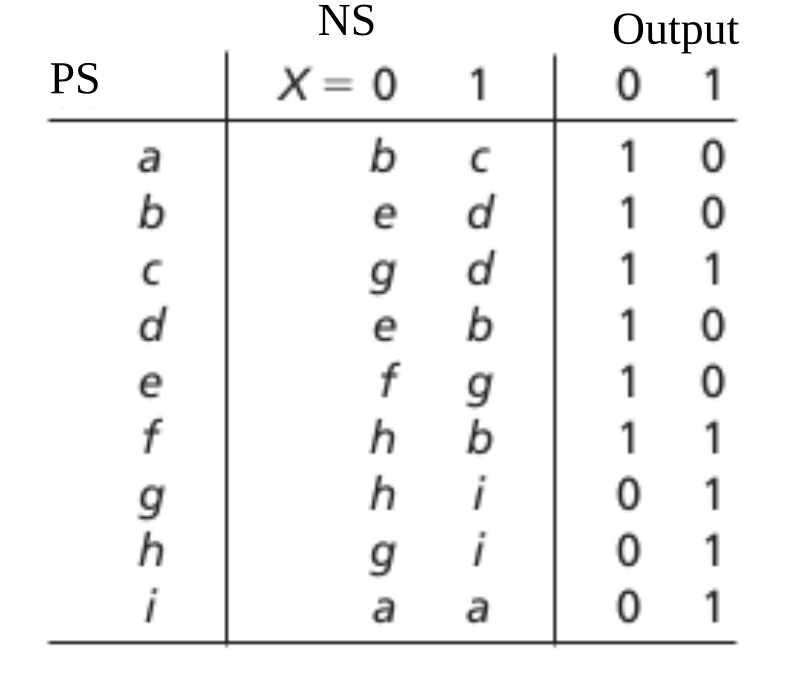
\includegraphics[width=0.3\linewidth]{./fig/15.15-state-table.png}
  \label{p:state-reduction}
\end{prob}
%\newpage

\begin{prob}
  % Reduce the following state table to a minimum number of states using
  % implication charts (20 marks).
  \begin{enumerate}
  \item
    Use the guideline method (Highest priority and Medium priority only) to determine a suitable \textbf{state assignment} for the state table (20 marks).
  % % \item
  % % Realize the table using D flip-flops.
  \item Realize the least significant bit of the encoding table using J-K flip-flops (30 marks).
  \end{enumerate} 

  \begin{tabular}{c|cc|c}
    \toprule
    Present State & \multicolumn{2}{c|}{Next State} & Output (Z)\\
                  & X = 0 & 1 & \\
                  \midrule
    A & A & B & 1\\
    B & C & E & 0\\
    C & F & G & 1\\
    D & C & A & 0\\
    E & B & G & 1\\
    F & F & B & 1\\
    G & C & F & 0\\
    \bottomrule
  \end{tabular}
\end{prob}
%\newpage

\begin{prob}
  A 4:2 priority encoder takes 4 inputs $y_0, y_1, y_2, y_3$ and has three outputs, $w_1, w_0$ and $\text{IST}$. Find boolean expressions for $w_1$ and $w_0$ using K-maps for the priority encoder. The priority encoder truth table is given for reference (``*'' indicates all possible input combinations and ``d'' indicates don't care output). (10 marks) \\
  \begin{tabular}{cccc|ccc}
    \toprule
    \multicolumn{4}{c|}{Inputs} & \multicolumn{3}{c}{Outputs}\\
    $y_0$ & $y_1$ & $y_2$ & $y_3$ & $w_1$ & $w_0$ & $\text{IST}$ \\
    \midrule
    0 & 0 & 0 & 0 & d & d & 0\\
    1 & * & * & * & 0 & 0 & 1\\
    0 & 1 & * & * & 0 & 1 & 1\\
    0 & 0 & 1 & * & 1 & 0 & 1\\
    0 & 0 & 0 & 1 & 1 & 1 & 1\\
    \midrule
  \end{tabular}
\end{prob}
%\newpage

\begin{prob}
  % 9 study guide 5
  (Optional for extra credit) The following diagram shows the pattern of 0’s and 1’s stored in a ROM
  with eight words and four bits per word. What will be the values of $F_1 , F_2 ,
  F_3 , and F_4$ if $A= B = 0$ and $C = 1$?
  Also give the minterm expansions for $F_1$ and $F_2$ (20 marks).\\
  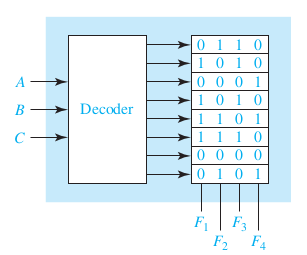
\includegraphics[width=0.4\linewidth]{./fig/ROM-minterms.png}
\end{prob}
%\newpage

\begin{prob}
  The following prime implicant table is for a four variable function $f(A, B,
  C, D)$.
  Give the algebraic expression of each of the essential prime implicants. Find
  the minimal sum of products expression for $f$ by PI table reduction. (10 marks)
  \\
  \begin{tabular}{ccccc}
    \toprule
    minterms \textbackslash PIs: & $\bB D$ & $\bB C$ & CD & AD  \\
    \midrule
    2  &   & $\times$ & & \\
    3  & $\times$ & $\times$ & $\times$ & \\ 
    7  &  & & $\times$ & \\ 
    9  & $\times$ & & & $\times$ \\ 
    11 & $\times$ & $\times$ & $\times$ & $\times$ \\ 
    13 &  & & & $\times$ \\
    \bottomrule
  \end{tabular}\\
\end{prob}
%\newpage

\begin{prob}
  Packages arrive at the stockroom and are delivered on carts to offices and laboratories
  by student employees.The carts and packages are various sizes and shapes.The students
  are paid according to the carts used. There are five carts and the pay for their use is\\
  Cart C1: \$2\\
  Cart C2: \$1\\
  Cart C3: \$4\\
  Cart C4: \$2\\
  Cart C5: \$2\\
  On a particular day, seven packages arrive, and they can be delivered using the five
  carts as follows:\\
  C1 can be used for packages P1, P3, and P4. \\
  C2 can be used for packages P2, P5, and P6. \\
  C3 can be used for packages P1, P2, P5, P6, and P7. \\
  C4 can be used for packages P3, P6, and P7. \\
  C5 can be used for packages P2 and P4. \\
  The stockroom manager wants the packages delivered at minimum cost. Using
  minimization techniques described in this class, present a systematic procedure for
  finding the minimum cost solution. (20 marks)
\end{prob}
%\newpage

\begin{prob}
  (a) For $V_{IH}$ = 4 V, $V_{OH}$ = 4.5 V, $V_{IL}$ = 1 V, $V_{OL}$ = 0.3 V, and $V_{DD}$ = 5 V, calculate the
  noise margins $NM_H$ and $NM_L$ (5 marks).\\
  (b) Draw an eight-input NAND gate built using NMOS technology and pull-up
  resistor (5 marks).\\
  (c) In the above circuit, if the voltage drop
  across each transistor is 0.1 V, what is $V_{OL}$ ? What is the corresponding $NM_L$ using the other
  parameters from part (a) (10 marks).
\end{prob}
%\newpage

\begin{prob}
  What is the difference between positive logic and negative logic? Design a
  CMOS complex gate for $f = x_1 \bx_2 + \bx_1 x_2$ under negative logic (10 marks).
\end{prob}
%\newpage

\begin{prob}
  Find the propagation delay and contamination  delay of the following circuit (5 marks):\\
  \includegraphics[width=0.4\linewidth]{./fig/fig2.83-circuit.png} 
\end{prob}
%\newpage

\begin{prob}
  Describe how tri-state and open-collector outputs are different from totem-
  pole outputs using NMOS NOR gate as an example (10 marks).
\end{prob}
%\newpage

% \begin{prob}
%   Assume that the inverter in the given circuit has a propagation delay of 5 ns and the
%   AND gate has a propagation delay of 10 ns. Draw a timing diagram for the circuit
%   showing X, Y, and Z. Assume that X is initially 0, Y is initially 1, after 10 ns X
%   becomes 1 for 80 ns, and then X is 0 again. (20 marks)\\
%   \includegraphics[width=0.4\linewidth]{./fig/fig-not-AND-latch.png}
% \end{prob}
%\newpage

\begin{prob}
  A latch can be constructed from an OR gate, an AND gate, and an inverter con-
  nected as follows: \\
  \includegraphics[width=0.4\linewidth]{./fig/or-AND-latch.png}\\
  \begin{enumerate}
    \item  What restriction must be placed on R and H so that P will always equal Q
    (under steady-state conditions) (10 marks)?
  \item Construct a characteristic (next-state) table and derive the
    corresponding characteristic equation for the latch (5 marks).
  \item Complete the following timing diagram for the latch (10 marks)\\
    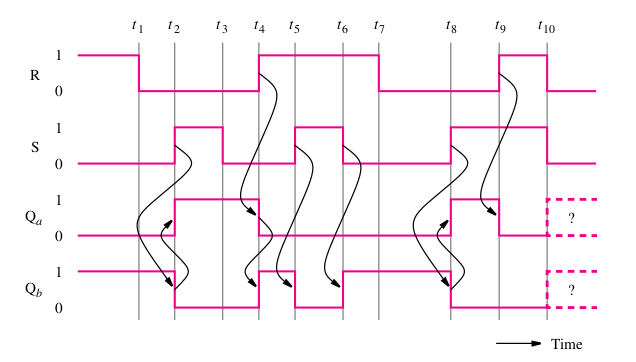
\includegraphics[width=0.4\linewidth]{./fig/timing-diagram.png}
  \end{enumerate}
\end{prob}
%\newpage

\begin{prob}
  Figure~\ref{fig:seven-seg-display} shows the notation for a BCD to 7-segment
display and Table~\ref{tab:seven-segment-tt} shows the corresponding truth
table. The inputs corresponding to the missing rows in the truth table should be
considered as don't care.
  \begin{enumerate}
   \item implement segment ``a'' using an 8:1 mux and no other logic gate, (10 marks)
   \item implement segment ``a'' using a 4:1 mux and one other gate, (10 marks)
   \item implement segment ``f'' with 4:1 mux and no other logic gate. Assume
     inputs are available in both uncomplemented and complemented form. (Hint:
     There are (${}^4C_2 = 6$) possible pairs of control inputs: ($w_3, w_2$), ($w_2, w_1$),
     ($w_1,w_0$), ($w_0, w_3$), ($w_0, w_2$), ($w_1, w_3$). There are 6 don't
     care conditions. With two control inputs of the multiplexer and one input,
     you can represent an expression with up to 4-SOP-terms of size
     three-literals or less. You might the arrive at the answer sooner, if you
     try to write the minimal SOP expression first and find the two inputs that
     occur most often in all the terms. Those two inputs are most likely to be the
     chosen pair of control inputs.) (10 marks)
  \end{enumerate}
\end{prob}

\begin{table}[h!]
  \footnotesize
\begin{tabular}{l|cccc||ccccccc}
  \toprule
  Row & $w_3$ & $w_2$ & $w_1$ & $w_0$ & a & b & c & d & e & f & g \\
  \midrule
  0  & 0    & 0   &   0 &   0 & 1 & 1 & 1 & 1 & 1 & 1 & 0 \\
  1  & 0    & 0   &   0 &   1 & 0 & 1 & 1 & 0 & 0 & 0 & 0 \\
  2  & 0    & 0   &   1 &   0 & 1 & 1 & 0 & 1 & 1 & 0 & 1 \\ 
  3  & 0    & 0   &   1 &   1 & 1 & 1 & 1 & 1 & 0 & 0 & 1 \\ 
  4  & 0    & 1   &   0 &   0 & 0 & 1 & 1 & 0 & 0 & 1 & 1 \\ 
  5  & 0    & 1   &   0 &   1 & 1 & 0 & 1 & 1 & 0 & 1 & 1 \\   
  6  & 0    & 1   &   1 &   0 & 1 & 0 & 1 & 1 & 1 & 1 & 1 \\ 
  7  & 0    & 1   &   1 &   1 & 1 & 1 & 1 & 0 & 0 & 0 & 0 \\ 
  8  & 1    & 0   &   0 &   0 & 1 & 1 & 1 & 1 & 1 & 1 & 1 \\
  9  & 1    & 0   &   0 &   1 & 1 & 1 & 1 & 1 & 0 & 1 & 1 \\
  \bottomrule
\end{tabular}
\caption{Truth table for BCD to seven-segment display as shown in
  Figure~\ref{fig:seven-seg-display}. The missing combinations of inputs should
  be considered as dont care.}
\label{tab:seven-segment-tt}
\end{table}

\begin{figure}[h!]
  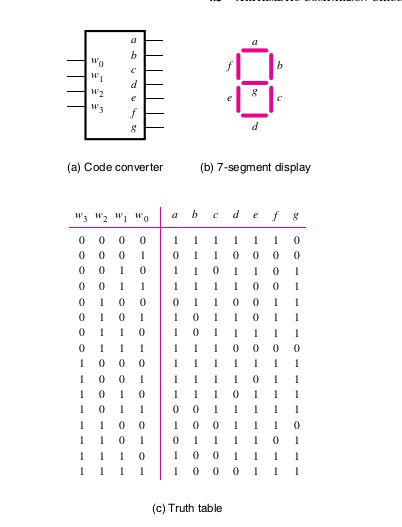
\includegraphics[width=\linewidth,trim=0 10cm 0 0.2cm,clip]{fig/fig-4.21.png}
  \\
  \caption{Seven segment display and BCD-to-7-segment display converter. When
    $a=1$ the corresponding segment of the display lights up. To display the
    number 8, you will turn on all the seven segments, while to display 1, you
    will turn on $b=1, c=1$ and turn off $=0$ the rest. The full truth-table for
  the seven-segment display is shown in Table~\ref{tab:seven-segment-tt}.}
  \label{fig:seven-seg-display}
\end{figure}

%\begin{prob}
%  Design a 4-bit BCD counter that counts from 0000, to 1001 and then loops back
%  to 0000 (20 marks).\\
%  \begin{enumerate}
%  \item Draw its state transition diagram and table
%  \item Design the circuit using a D flip-flop.
%  \end{enumerate}
%\end{prob}
%\newpage

\begin{prob}
  Design a 3-bit modulo 8 Gray counter that counts from 000, to 111 and then loops back
  to 0000. (A modulo N counter counts from 0 to $N-1$) (20 marks).\\
  \begin{enumerate}
  \item Draw its state transition table
  \item Design the circuit using a D flip-flop.
  \end{enumerate}
\end{prob}


%\bibliography{main}
%\bibliographystyle{plain}
\end{document}
